\documentclass{article}
\usepackage[english]{babel}
\usepackage{fullpage}
\usepackage{color}
\usepackage{url}
\usepackage[parfill]{parskip}
\usepackage[pdftex]{graphicx}
\usepackage{hyperref}
\usepackage[nonumberlist]{glossaries}
\makeglossaries

\newcommand{\maakgls}[2]{\newglossaryentry{#1}{name=#1,description={#2}}}

\maakgls{binary}{An attribute that can have only two distinct values. These
values will be represented in Cortana with 0 and 1. Cortana will form
subgroups \emph{attr}=0 and \emph{attr}=1}
\maakgls{nominal}{An attribute that can have any countable number of
distinct values.  No ordering is assumed between these values.  Cortana will
form subgroups \emph{attr}=\emph{value}, and \emph{attr}$\neq$\emph{value}
when the ``include $\neq$ (nominal)'' checkbox in the Search Strategy Panel
is selected (see Section \ref{sec:searchstrategy})}
\maakgls{ordinal}{An attribute that can have any countable number of
distinct values. A natural ordering exists between these values. Cortana
cannot handle this attribute type. Depending on which kind of subgroups you
would want to consider, you can make Cortana handle such an attribute as
either \gls{nominal} or \gls{numeric}}
\maakgls{numeric}{An attribute that can have values from a continuous range. 
Cortana will form subgroups \emph{attr}$\leq$\emph{value} and
\emph{attr}$\geq$\emph{value}.  You can control how many and which values
will be selected in the Search Strategy Panel (see Section
\ref{sec:searchstrategy})}
\maakgls{type}{Determines the range of values an attribute can have. In
Cortana, an attribute can have types \gls{binary}, \gls{nominal}, or
\gls{numeric}.  Attributes in Cortana cannot be \gls{ordinal}; for these
attributes you can either select the \gls{nominal} or \gls{numeric} type,
depending on what kind of subgroups you would like to see}
\maakgls{enabled}{An attribute that will be considered for
generating candidate subgroups}
\maakgls{disabled}{An attribute that will not be considered for
generating candidate subgroups}

\title{Cortana for Dummies}
\author{Marvin Meeng, Wouter Duivesteijn}
\date{December 6, 2012}

\newcommand{\todo}[1]{\textcolor{red}{[TODO: #1]}}

\begin{document}
\maketitle

\section{What is Cortana, and what does it do?}
\label{sec:intro}

Cortana is a tool which, given a dataset, performs Supervised Descriptive
Local Pattern Mining:
\begin{description}
\item[Local Pattern Mining:] a run of Cortana strives to find \emph{subsets}
of the dataset where \emph{something interesting} is going on. We try to
pinpoint local exceptionalities in your dataset.
\item[Descriptive:] subsets delivered by Cortana are not just any subsets of
the data, but \emph{coherent} subsets, defined on attributes. Such subsets
are called \emph{subgroups}.
\item[Supervised:] the interestingness is measured with respect to a
user-defined \emph{target concept}: a subset of attributes that we are
particularly interested in. Cortana finds subgroups for which the target
concept is substantially different than the target concept over the entire
dataset.
\end{description}

As an example,
%of the things Cortana could find, 
suppose a dataset about people, and let the target concept be the
distribution of just one binary attribute: whether the person develops lung
cancer or not.  Cortana can find subgroups like \emph{smoking = true} (the
smokers, which have a substantially higher incidence of lung cancer), and
\emph{weekly walking kilometers} $\geq 50$ (athletes, which have a
substantially lower incidence of lung cancer).
\todo{might need a better example here}

\section{Launching Cortana}

After obtaining and unpacking a copy of Cortana from
\url{http://datamining.liacs.nl/cortana.html}, navigate to the Cortana
directory where you will find a cortana.jar file.  One could start Cortana
by double clicking the jar.  However, it is recommended to start Cortana
from the command line, since this will feed back information information
about the Subgroup Discovery process to the user.  To start Cortana this
way, open a terminal or command window, navigate to the Cortana directory
containing cortana.jar, and type: \emph{java -jar cortana.jar}. 
Alternatively, one can use either cortana.bat (for Windows) or cortana.sh
(Bash shell script).  Be sure to read Appendix~\ref{sec:memory} if your
computer displays memory issues while running Cortana.

After starting Cortana you are prompted for the file containing the dataset
to be analysed, after which Cortana's main screen is shown.

Cortana can handle two kinds of files: ARFF files and
plain (comma seperated) text files.  
An ARFF file combines the data with definitions of the \gls{type} of
each attribute.  
%As such, ARFF files are preferred over plain text files. 
For text files, Cortana wil try to automatically infer these \gls{type}s.
Unfortunately, this may not always deliver the desired outcome.  We will
discuss how to correct wrong assessments in Section \ref{sec:metadata}, but
in order to prevent the problem, we recommend the use of ARFF files when
this option is available.

\section{Main Screen}

\begin{figure}
\begin{center}
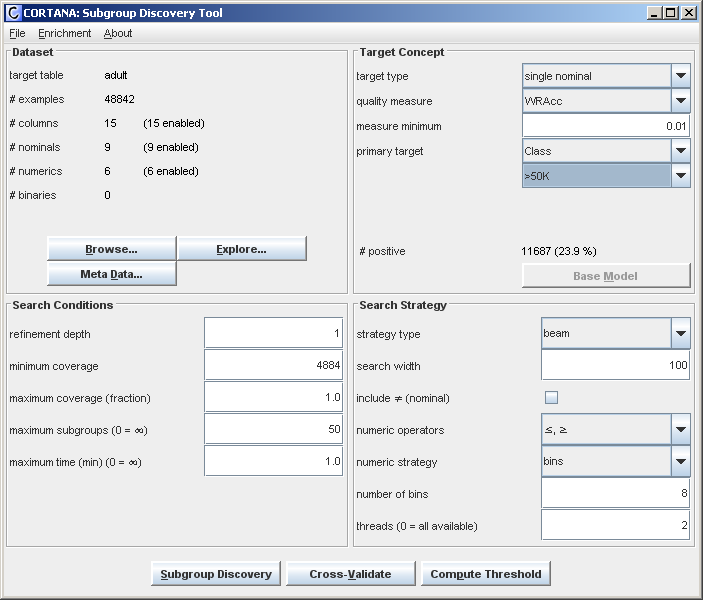
\includegraphics[width=\textwidth]{miningwindow_r1011.png}
\caption{Cortana's main window.}
\label{fig:mainwindow}
\end{center}
\end{figure}

The main screen of Cortana is devided into four major panels,
\emph{Dataset}, \emph{Target Concept}, \emph{Search Conditions}, and
\emph{Search Strategy}.

\subsection{Dataset Panel}
\label{sec:dataset}

%\begin{figure}
%\begin{center}
%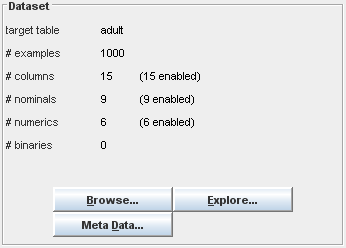
\includegraphics[width=0.5\textwidth]{dataset.png}
%\caption{Dataset details in the main window.}
%\end{center}
%\label{fig:dataset}
%\end{figure}

The Dataset panel contains information about the dataset that is currently
loaded:
\begin{description}
\item[target table] shows the name of the data file used. For text
files this is the filename, and for ARFF files this is the name defined in the
`@relation' field;
\item[\# examples] shows the number of examples in the dataset;
\item[\# columns] shows the number of columns in the dataset.
Remember that columns are also be referred to as attributes.
\end{description}
Finally, there is a number of fields that indicate the number of attributes
from each \gls{type}: \gls{nominal}, \gls{numeric}, and \gls{binary}. Notice
that Cortana cannot handle \gls{ordinal} data; such attributes can be
handled as either \gls{nominal} or \gls{numeric}, depending on what kind of
subgroups you would want to define on the attribute.

In addition to the fields described above, there are three buttons present
on the {\bf Dataset} panel: {\bf Browse\ldots}, {\bf Meta Data\ldots} and
{\bf Explore\ldots}.

\subsubsection{Browse Window}

Clicking the Browse button will open a Browse Window, displaying the
data in its current state.  You can sort the data by clicking on the column
head of an attribute, and save the current state of the data to a file,
which is useful if you have made modifications via the Meta Data Window (see
Section \ref{sec:metadata}).

%\begin{figure}
%\begin{center}
%\centering
%\resizebox{1\columnwidth}{!}{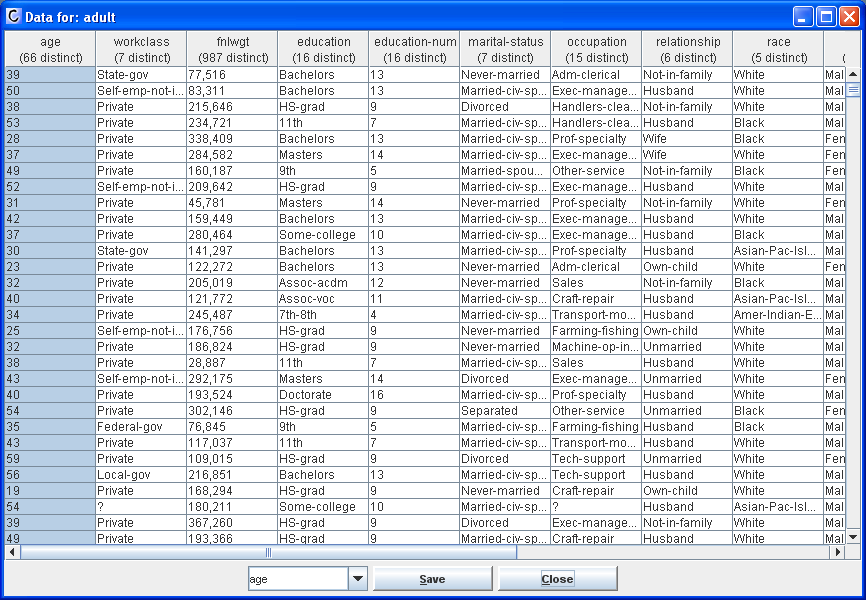
\includegraphics{browsewindow.png}}
%\caption{The browse window.}
%\end{center}
%\label{fig:browsewindow}
%\end{figure}

%By clicking the {\bf Browse...} button, a Browse Window is presented, showing a table with the data in
%its current state.
%Additionally, in the table header, it shows the number of distinct values for each attribute.
%Note that the data may not be in the same state as when it was loaded, as it can be modified using functionality of the Meta Data Window, presented after pressing the {\bf Meta Data...} button, which is also present on the {\bf Dataset} panel.
%Section~\ref{sec:metadata} describes the Meta Data Window, its components, and the data manipulation functionalities, in more detail.

\subsubsection{Explore Window}

Clicking the Explore button will open an Explore Window, which allows you to
examine the distribution of single attributes, and cross-examine two
attributes.  This section of Cortana is independent of the Local Pattern
Mining for which Cortana was developed; it exists merely to allow you to
learn more about the makeup of your data.

\subsubsection{Meta Data Window}
\label{sec:metadata}

\begin{figure}
\begin{center}
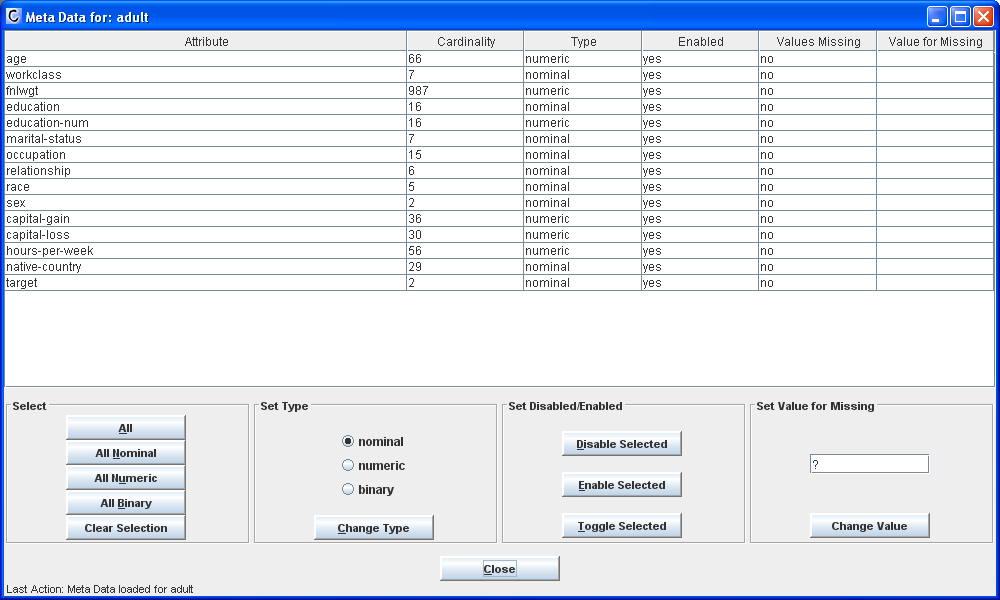
\includegraphics[width=\columnwidth]{metadatawindow.png}
\caption{Meta data window.}
\end{center}
\label{fig:metadatawindow}
\end{figure}

Clicking the Meta Data button will open a MetaData window, which displays
information on the attributes of the current dataset and allows changing
some of the attribute properties.  The upper part of the window shows a
table with six columns.  The lower part contains a number of panels that
allow modification of the data as it is in memory.  Note that no
modifications are made to the original data file.  First the properties
shown in the table in the upper part will be described, the purpose of the
various data manipulations will be explained after that.

\paragraph{Meta Data Table}
\label{meta-data-window:meta-data-table}

The upper part of the MetaData window displays a table containing the current
attribute information.  The first column in this table, \emph{Attribute},
lists the attribute names.  \emph{Cardiality} gives the number of distinct
values for the attribute.  \emph{Type} shows its attribute \gls{type}. 
\emph{Enabled} indicates whether the attribute is \gls{enabled} or
\gls{disabled}; this setting affects the search for subgroups, which will be
discussed in Section \ref{sec:searchstrategy}.  \emph{Values Missing}
indicates whether values for the attribute are missing in the dataset, and
if so, \emph{Value for Missing} shows the value that is currently used for
these missing values.  If not, this field is blank.

\paragraph{Meta Data Functions}
\label{meta-data-window:meta-data-functions}

The panels in the lower part of the \emph{Meta Data Window} all allow
selecting or changing the data.  The first, \emph{Select}, allows selecting
all attributes of a certain type.  This is a convenience method to be used
in combination with the functionalities available in other panels.

\subparagraph{Set Type} allows changing the attribute \gls{type}.  Cortana
makes an educated guess which \gls{type} each attribute should have. 
Occasionally you will want to change this assessment, and if possible
this panel will allow it.  Select the attributes in the table in the upper
part of the MetaData window, choose the radio button corresponding to the
desired type, and click the Change Type button.  If the requested action can
be performed, Cortana will do so, and if not (for instance: if you try to
make an attribute binary while it has more than two distinct values),
Cortana will do nothing.

%This can be useful for various reasons.  The first is that, after loading a
%plain text file, it is observed that Cortana was not capable to infer the
%correct type for an attribute.  Related to this is the possiblity to change
%the type of an attribute to allow other quality measures to be used in the
%Subgroup Discovery process.  An example of this would be an attribute that
%describes the number of doors in a car dataset.  If this value is used as a
%target value, one might treat it as a \emph{nominal} property, forcing the
%Subgroup Discovery process to only perform equality tests on this
%\emph{attribute value} for the creation of the conditions used to form
%subgroups.  \emph{Instances} in the dataset are then either in the target
%set if they have the same value for the `doors' attribute as the selected
%target value, or are in the complement of the set formed by those instances. 
%If the `doors' attribute is treated as \emph{numeric}, any, combination, of
%the `$<=$', `$>=$' and `$=$' tests can used to create conditions to perform
%on the \emph{attribute values}.  This means that the size of the set of
%instances selected using an \emph{attribute value} might be bigger than in
%the \emph{nominal} case.  A condition using $doors >= 2$ will select all
%cars having two or more doors.  In the \emph{nominal} case it would not be
%possible to select this group using only one condition (assuming the set of
%cars having more than two doors is not empty).  Obviously, it would be
%possible to select the same group using a set of conditions like $doors
%equals `2' \vee doors equals `3' \ldots$, but, among other negative
%characteristics, creating such conditions would be computationally more
%demanding, and less intuitive.  Note that if there are missing values for an
%attribute, the \emph{missing value} value for this attribute might be
%automaticaly changed to a value that is relevant to the attribute type.  See
%\emph{Set Value for Missing} below for more on the \emph{missing value}
%values for the different attribute types.
%\ref{subsubsection:set-missing-values}

\subparagraph{Set Disabled/Enabled} allows to disable or enable an
attribute. The relevance of this choice will be discussed in
Section~\ref{sec:searchstrategy}; by default all attributes are enabled.

%When an attribute is disabled, it will not be considered by the mining
%algorithm to form conditions with to create subgroups.  Note that disabling
%an attribute does not affect the possiblity to select it as a target concept
%(see section~\ref{sec:targetconcept} for more on target concepts).

\subparagraph{Set Value for Missing} can be used to change the value that is
currently used as a proxy for missing occurrences of this attribute in the
data. Details can be found in the Full Cortana Manual.

%\todo{several spelling errors in the following paragraph. Haven't corrected
%them, since they're commented out anyway.}
%\subparagraph{Set Value for Missing} can be used to change the value that is
%currently used as a proxy for missing occurences of this attribute in the
%data.  The default value that is used for missing values depends on the
%attribute type.  If, in an ARFF file, values are declared missing using
%the `\emph{?}' directive, Cortana's file loader might replace this value
%with one that makes more sense in its Subgroup Discovery setting.  For
%\emph{nominal} types it will leave this value as is.  This will result in
%`\emph{?}' being one of the possible target values one can select for the
%corresponding attribute.  However, one can assign a diffent value to the
%\emph{missing values}.  One than has two options, either assign the
%\emph{missing values} a value that is an existing one for the attribute, or
%a non-exiting one.  In the first case one effectively assigns all instances
%that have a missing value for the corresponding attribute to one of the
%other \emph{attribute values}.  In the latter case, one just changes the
%value.  When changing the \emph{missing value} value of an attribute, the
%\emph{Cardinality} column is updated accordingly.  For \emph{numeric} and
%\emph{binary} attribute types Cortana's file loader will replace `\emph{?}'
%values with $0.0$ and $false$, respectively.  Again, if this is incorrect,
%or one wishes to assign the \emph{missing values} another \emph{attribute
%value}, either existing or non-existing, this can be done analogously to the
%\emph{nominal} case.

\subsection{Target Concept Panel}
\label{sec:targetconcept}

The settings in the Target Concept panel determine how the Cortana process
is \emph{supervised}, as described in Section \ref{sec:intro}.  A Cortana
run strives to find subgroups for which a target concept is substantially
different than the target concept over the entire dataset.  In the Cortana
Light Manual, we will focus on the case where this target concept is the
distribution of a single attribute.  Cortana can also find subgroups for
more complex target concepts; these are described in the Full Cortana
Manual.

Since the \gls{type} of the target attribute determines the number of
parameters to be set, you have to indicate it first.  Hence, the first
drop-down menu in the Target Concept panel is {\bf target type}, which more
generally determines what sort of target concept we are interested in.  The
\emph{single nominal} and \emph{single numeric} choices correspond to having
one single target attribute, either nominal or numeric.

When the target attribute type is \gls{nominal}, you have to set four
additional parameters.  In the third drop-down menu (\textbf{primary
target}) of the Target Concept panel, you can select the target attribute,
and in the fourth drop-down menu, you can select the desired value for that
target (i.e.\@ the value for which you want to see an increase or
decrease in the found subgroups).  
The second drop-down menu (\textbf{quality measure}) lists the available
quality measures.  The default selection, ``WRAcc'', will only search for
subgroups with an increased presence of the target value.  If you are also
interested in subgroups with a decreased presence of the target value, you
can select either ``Abs WRAcc'' or ``Chi-squared''. Directly below the
quality measure drop-down menu, you find a field where you can enter the
minimal quality value a subgroup must have (\textbf{measure minimum}).
Usually the default value should do, but if your subgroup discovery run
provides no results, a lower measure minimum might help.

When the target attribute type is \gls{numeric}, you have to set three
additional parameters.  In the third drop-down menu (\textbf{primary
target}) of the Target Concept panel, we have to select the target
attribute.  Unlike in the nominal case, there is not one particular value
for the attribute to be interested in; instead we search for subgroups with
relatively high or relatively low values for the target.  The second
drop-down menu (\textbf{quality measure}) lists the available quality
measures.  The default selection, ``Z-Score'', will only search for
subgroups with a relatively high average target value.  If you are
interested in subgroups with a relatively low average target value, you can
select ``Inverse Z-Score'', and if you are interested in both, you can
select or ``Abs Z-Score''.  Again, directly below the quality measure
drop-down menu, you can set the \textbf{measure minimum}, and again, usually
the default value should do, but if your subgroup discovery run provides no
results, a lower measure minimum might help.

\subsection{Search Conditions Panel}
\label{sec:searchconditions}

The fields in the Search Conditions panel allow setting the search
conditions used in the Subgroup Discovery process.  The process is discussed
in detail in Section \ref{sec:searchprocess}.

\textbf{refinement depth} controls the number of conditions that is used to
define subgroups.  A refinement depth of $1$ would lead to subgroups of the
form $x \leq 9.11$, while a refinement depth of $2$ would allow for
subgroups of the form $x \leq 1.2 \wedge y \geq 3.4$.  It is not recommended
to set the refinement depth to very high values.  Usually, the added
conditions on depth $4$ or $5$ and beyond do not substantially contribute to
subgroups, but merely make them harder to interpret while the increased
depth does substantially add computational time needed to calculate the
result.

\textbf{minimum coverage} sets the lower bound for the size of the subgroups
that should be reported by Cortana, meaning all reported subgroups have at
least this size.  The default value is $10\%$ of the dataset size.

\textbf{coverage fraction} sets the upper bound for the size of the
subgroups that should be reported by Cortana, meaning all reported subgroups
have at most this size.  The default value is set to $1.0$, which allows
subgroups to encompass the entire dataset.

\textbf{maximum subgroups} is used to control the maximum number of
subgroups in the result list generated by Cortana.  Setting this parameter
to $0$ allows Cortana to report all found subgroups.

\textbf{maximum time (min)} is used to control the maximum time, measured in
minutes, Cortana is allowed to search for new subgroups.  If the time limit
is reached, Cortana will abort the Subgroup Discovery process and report all
subgroups found so far.  Usually this means that a substantial part of the
search space will not be explored at all.  You can set this parameter to $0$
to allow Cortana as much time as necessary.

\subsection{Search Strategy Panel}
\label{sec:searchstrategy}

The Search Strategy panel determines the terms under which the search
process is carried out.  Usually the default values will do, apart maybe
from the search width and the operator selection parameters. To fully grasp
the impact of these parameters, you might want to read about the search
process (Section \ref{sec:searchprocess}) first, and revisit this section
afterwards.

\textbf{strategy type} allows you to set the overarching search strategy. 
In this manual we will focus on the ``beam'' setting; for more on the other
strategies, please see the Full Cortana Manual.  If you find the reported
subgroups that Cortana too similar to each other, you could alternatively
try the ``cover-based beam selection'' setting.

\textbf{search width} sets the beam width. See Section
\ref{sec:searchprocess} for details.

\textbf{include $\neq$ (nominal)} determines the subgroups considered for
each nominal attribute.  When unchecked, on each nominal attribute only
subgroups of the form \emph{attr}$=$\emph{value} will be considered.  When
checked, \emph{additionally} subgroups of the form
\emph{attr}$\neq$\emph{value} will be considered.

Together, \textbf{numeric operators}, \textbf{numeric strategy}, and
\textbf{number of bins} determine the subgroups considered for each numeric
attribute.  Usually, the default selection will do.  For more details, see
the Full Cortana Manual.

\textbf{threads} sets the number of hyperthreads used on your computer for
the Cortana process.  When you run Cortana on a multi-core system,
increasing this number will reduce the time necessary to complete the
process.  You can set the parameter to $0$ to allow Cortana to use every
available hyperthread.

\section{The Search Process}
\label{sec:searchprocess}

\section{Result Window}
\label{section:result-window}

\appendix
\clearpage
~\vfill

\resizebox{\textwidth}{!}{Appendices}

\vfill~
\clearpage

\section{Glossary}
\vspace{-10mm}
\renewcommand*{\glossaryname}{}
\printglossaries

\section{Autorun}

\section{Memory Issues}
\label{sec:memory}

Although Cortana is written in Java, and therefore platform independent, it will behave slightly different on different operation systems and/or platforms.
These differences arise from small variations in the Java Virtual Machines, used in different situations.
The main issue is with 32-bit operating systems (OS).
On such systems the maximum amount of memory the Java Virtual Machine (JVM) can use is around 1600 MegaBytes.
However, the actual amount depends on the amount of RAM available.
The cortana.bat and cortana.sh file included in the Cortana.zip set the maximum amount of memory the JVM can use to 1600 MegaBytes, through the -Xmx option.
The value should, at most, be set to half the amount of available RAM, meaning eg. for a 2GB machine to \emph{-Xmx1000m}.
For 64-bit OSes no such limit exists, and it should be save to remove the -Xmx.
Note that the above means that, especially for 32-bit OSes, not all datasets will fit into memory.

\end{document}
